Zuerst    wurde    die    Brennweite    von    Linse    $L_1$    experimentell
\"uberpr\"uft. Anschliessend wurde die Str\"omungsgeschwindigkeit in der Mitte
des  Messohres  f\"ur  verschiedene Durchflussraten  gemessen. Zuletzt  wurden
die  Str\"omungsprofile f\"ur  den  laminaren Fall  und  den turbulenten  Fall
aufgenommen.

% ---------------------------------------------------------------------------- $
\subsection{Schnittwinkel der Laserstrahlen}
\label{subsec:varphi}
% ---------------------------------------------------------------------------- $

Die Brennweite der Linsen sind zwar angegeben, wir wollen uns aber nicht darauf
verlassen, und diese experimentell \"uberpr\"ufen. Daraus ergibt sich dann auch
der Schnittwinkel $\varphi$ der Laserstrahlen.

 Es wurden die Distanzen $d_L$ zwischen  den beiden Strahlen beim Eintreten in
die Linse und die Distanz $d_f$  zwischen der Linse und dem Kreuzungspunkt der
Laserstrahlen gemessen. Die  Bestimmung des  Schnittwinkels ist dann  nur noch
eine Sache von ein wenig Trigonometrie.

F\"ur   die  Distanzen   ergaben  sich   folgende  Werte,   mit  gesch\"atzten
Unsicherheiten:

\begin{itemize}
    \item
        $ d_L = \SI{52.5 \pm 0.5}{\milli\meter}$
    \item
        $ d_f = \SI{130 \pm 1}{\milli\meter}$
\end{itemize}

Der halbe Schnittwinkel ergibt sich dann zu:

\begin{equation}
    \label{eq:varphi_half}
    \frac{\varphi}{2} = \arctan \frac{\frac{d_L}{2}}{d_f}
\end{equation}

Der kleinstm\"ogliche Winkel ergibt sich aus der Kombination von
$d_L = \SI{52}{\milli\meter}$
und
$d_f = \SI{131}{\milli\meter}$
und
bel\"auft sich auf
$\frac{\varphi}{2} = \SI{11.23}{\degree}$,
der gr\"osstm\"ogliche Winkel korrespondiert mit
$d_L = \SI{53}{\milli\meter}$
und
$d_f = \SI{129}{\milli\meter}$
und ergibt
$\frac{\varphi}{2} = \SI{11.61}{\degree}$,
was sich zusammenf\"uhren l\"asst auf einen Schnittwinkel von:

\begin{equation}
    \label{eq:varphi_result}
    \varphi = \SI{11.42 \pm 0.19}{\degree} \cdot 2 = \SI{22.8 \pm 0.4}{\degree}
\end{equation}

Der Vorgang ist ist schematisch in Abbildung \ref{fig:varphi} dargestellt.

\begin{minipage}[t]{\textwidth}
    \centering
    \resizebox{.67\textwidth}{!}{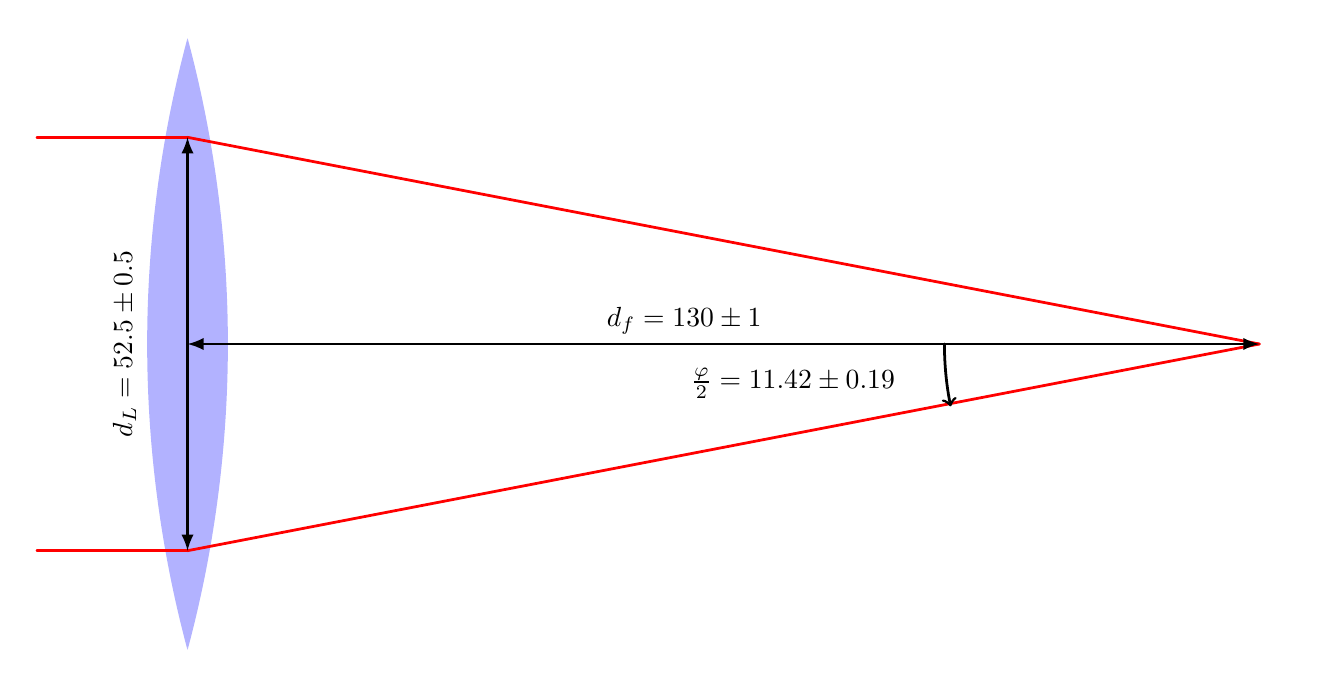
\begin{tikzpicture}
    \begin{scope}[x={(0mm,160mm)},y={(-40mm,40mm)},line width=1pt,cap=round]
        % bounding box
        \draw[white] (0mm,-40mm) rectangle (160mm,40mm);
        %\draw[-] (0mm,-30mm) -- (150mm,30mm);

        % Lens. Center: 20.125mm,0mm
        \fill[-,blue!30] (15mm,   0mm) -- (25.25mm,0mm) arc[start angle=0,  delta angle=15, radius=150mm] -- cycle;
        \fill[-,blue!30] (15mm,   0mm) -- (25.25mm,0mm) arc[start angle=0,  delta angle=-15,radius=150mm] -- cycle;
        \fill[-,blue!30] (25.25mm,0mm) -- (15mm,   0mm) arc[start angle=180,delta angle=15, radius=150mm] -- cycle;
        \fill[-,blue!30] (25.25mm,0mm) -- (15mm,   0mm) arc[start angle=180,delta angle=-15,radius=150mm] -- cycle;

        % incoming laser beams
        \draw[-,red] (1mm, 26.25mm) -- (20.125mm, 26.25mm);
        \draw[-,red] (1mm,-26.25mm) -- (20.125mm,-26.25mm);

        % outgoing laser beams
        \draw[-,red] (20.125mm, 26.25mm) -- (156.25mm,0mm);
        \draw[-,red] (20.125mm,-26.25mm) -- (156.25mm,0mm);

        % measurement arrow
        \draw[latex-latex,black] (20.125mm,0mm) -- (156.25mm,0mm);
        \draw[latex-latex,black] (20.125mm,-26.25mm) -- (20.125mm,26.25mm);
        \node[rotate=90] at (12.125mm,0mm) {$ d_L = \SI{52.5 \pm 0.5}{\milli\meter}$};
        \node at (83.2mm,3mm) {$ d_f = \SI{130 \pm 1}{\milli\meter}$};

        % angle arc
        \draw[->] (116.25mm,0mm) arc[start angle=180, delta angle=11.41, radius=40mm];
        \node at (97mm,-5mm) {$\frac{\varphi}{2} = \SI{11.42 \pm 0.19}{\degree}$};
    \end{scope}
\end{tikzpicture}
}
    \captionof{figure}{%
        Bestimmung des Schnittwinkels der  Laserstrahlen aus der Geometrie der
        Versuchsanordnung.  \emph{Beachte:} Da  diese Abbildung  prim\"ar  der
        Illustration  der Bestimmung  von  $\varphi$ und  nicht der  akkuraten
        Darstellung der Linse  dient, ist hier nicht das  gleiche Symbol f\"ur
        die Linse wie in der Versuchsanleitung benutzt worden.%
    }
    \label{fig:varphi}
\end{minipage}


% ---------------------------------------------------------------------------- $
\subsection{Str\"omungsgeschwindigkeit auf Achse der Messleitung}
\label{subsec:achse}
% ---------------------------------------------------------------------------- $

Gemessen wurden zwar Frequenzen, es sollen in den Regressionen jedoch direkt die
zugeh\"origen Geschwindigkeiten angegeben werden. Diese k\"onnen mit der folgenden
Formel ermittelt werden:

\begin{equation}
    \begin{split}
        \label{eq:deltaF2}
        \Delta\,f &= f_0 \cdot \frac{2 \cdot v}{c} \cdot \sin\left( \frac{\varphi}{2}\right) \\
                  &= \frac{c}{\lambda_{Laser}} \cdot \frac{2 \cdot v}{c} \cdot \sin\left( \frac{\varphi}{2}\right)\\
                  &= \frac{2 \cdot v}{\lambda_{Laser}} \cdot \sin\left( \frac{\varphi}{2}\right)
    \end{split}
\end{equation}

Aufgel\"ost nach $v$ ergibt dies:
\begin{equation}
    \label{eq:vFromf}
    v = \frac{\Delta\,f \cdot \lambda_{Laser}}{2 \cdot \sin\left(\frac{\varphi}{2}\right)}
\end{equation}


\begin{conditions}
    v               & Flussgeschwindigkeit des Streuteilchens \\
    \Delta\,f       & Gemessene Streufrequenz                 \\
    \lambda_{Laser} & Wellenl\"ange des Lasers                \\
    \varphi         & Kreuzungswinkel der Laserstrahlen (\SI{22.8 \pm 0.4}{\degree} gem\"ass vorigem Abschnitt) \\
\end{conditions}

Da die Flussgeschwindigkeit  $v$ f\"ur die Auswertung  selbst verwendet werden
soll, werden  zur besseren Leserlichkeit  hier auch gleich  die entsprechenden
Unsicherheiten bestimmt, anstatt diese in ein separates Kapitel auszulagern.

Es  sind  hier   sowohl  Unsicherheiten  im  Winkel  $\varphi$   wie  auch  in
der  gemessenen  Frequenz  vorhanden. Somit   ist  f\"ur  die  Bestimmung  der
Unsicherheit  der  Teilchengeschwindigkeit   die  Verwendung  des  Gauss'schen
Fehlerfortpflanzungsgesetzes erforderlich. Zur Erinnerung:

\begin{equation}
    \label{eq:Gauss}
    %\begin{split}
    s_{\overline{R}} = \sqrt{ \left( \frac{\partial R}{\partial x} \biggr\rvert_{\overline{R}} \cdot s_{\overline{x}}\right)^2
                            + \left( \frac{\partial R}{\partial y} \biggr\rvert_{\overline{R}} \cdot s_{\overline{y}}\right)^2
                            + \left( \frac{\partial R}{\partial z} \biggr\rvert_{\overline{R}} \cdot s_{\overline{z}}\right)^2
                            + ... }
    %\end{split}
\end{equation}

Angewandt auf die Formel der Teilchengeschwindigkeit:

\begin{equation}
    \label{eq:gauss:teilchen}
    \begin{split}
        s_{\overline{v}} = \sqrt{ \left( \frac{\partial v}{\partial f}       \biggr\rvert_{\overline{v}}       \cdot s_{\overline{f}}       \right)^2
                                + \left( \frac{\partial v}{\partial \varphi} \biggr\rvert_{\overline{\varphi}} \cdot s_{\overline{\varphi}} \right)^2
                                } \\
    \end{split}
\end{equation}

Mit:
\begin{align}
    \label{eq:partials}
    \frac{\partial v}{\partial f}       &= \frac{\lambda}{2 \cdot \sin \left( \frac{\varphi}{2} \right) } \\
    \frac{\partial v}{\partial \varphi} &= \frac{-f \cdot \lambda \cdot \cos\left(\frac{\varphi}{2}\right)}{4 \cdot \sin^2\left(\frac{\varphi}{2}\right)}
\end{align}

Ergibt sich somit:
\begin{equation}
    \label{eq:gauss:teilchen:eingesetzt}
    s_{\overline{v}} = \sqrt{ \left( \frac{\lambda}                                                    {2 \cdot \sin  \left( \frac{\varphi}{2} \right)} \biggr\rvert_{\overline{v}}       \cdot s_{\overline{f}}       \right)^2
                            + \left( \frac{-f \cdot \lambda \cdot \cos\left( \frac{\varphi}{2} \right)}{4 \cdot \sin^2\left( \frac{\varphi}{2} \right)} \biggr\rvert_{\overline{\varphi}} \cdot s_{\overline{\varphi}} \right)^2
                            }
\end{equation}

Formel   \ref{eq:gauss:teilchen:eingesetzt}  und   die  Messwerte   wurden  in
einem  Python-Script  ausgewertet,  das in  Anhang  \ref{app:python:rohrmitte}
auf  Seite \pageref{app:python:rohrmitte}  zu  finden ist. Die  resultierenden
Flussgeschwindigkeiten    mit   ihren    Unsicherheiten   sind    in   Tabelle
\ref{tab:rohrmitte} zu finden.

\begin{table}[h!t]
    \centering
    \caption{Messwerte f\"ur verschiedene Durchflussraten in Rohrmitte}
    \label{tab:rohrmitte}
    \begin{tabular}{SSSSSS}
        \toprule
        {$\dot{V}$ (\si{\liter\per\minute})}
        & {$f_{low}$ (\si{\kilo\hertz})}
        & {$f_{high}$ (\si{\kilo\hertz})}
        & {$\overline{f}$ (\si{\kilo\hertz})}
        & {$s_{\overline{f}}$ (\si{\kilo\hertz})}
        & {$v$ (\si{\centi\meter\per\second})}
        \\

        \midrule

        0.5
        & 7.07
        & 7.71
        & 7.39
        & 0.32
        & 2.4 \pm 0.1
        \\

        1.01
        & 13.43
        & 14.38
        & 13.905
        & 0.475
        & 4.4 \pm 0.2
        \\

        1.52
        & 17.59
        & 19.77
        & 18.68
        & 1.09
        & 5.9 \pm 0.4
        \\

        2.02
        & 23.19
        & 25.32
        & 24.255
        & 1.065
        & 7.7 \pm 0.4
        \\

        2.5
        & 26.66
        & 30.29
        & 28.475
        & 1.815
        & 9.1 \pm 0.6
        \\

        3.0
        & 30.18
        & 35.09
        & 32.585
        & 2.505
        & 10.4 \pm 0.8
        \\

        3.5
        & 34.85
        & 39.3
        & 37.075
        & 2.225
        & 11.8 \pm 0.7
        \\

        4.0
        & 36.21
        & 43.12
        & 39.665
        & 3.455
        & 12.6 \pm 1.1
        \\

        4.5
        & 40.95
        & 49.48
        & 45.215
        & 4.265
        & 14.4 \pm 1.4
        \\

        5.0
        & 45.51
        & 52.75
        & 49.13
        & 3.62
        & 15.6 \pm 1.2
        \\

        5.5
        & 51.34
        & 58.30
        & 54.82
        & 3.48
        & 17.4 \pm 1.1
        \\

        6.0
        & 57.16
        & 61.91
        & 59.535
        & 2.375
        & 18.9 \pm 0.8
        \\

        6.5
        & 60.78
        & 70.84
        & 65.81
        & 5.03
        & 20.9 \pm 1.6
        \\

        7.0
        & 64.44
        & 72.48
        & 68.46
        & 4.02
        & 21.8 \pm 1.3
        \\

        7.5
        & 67.12
        & 77.42
        & 72.27
        & 5.15
        & 23.0 \pm 1.7
        \\

        \bottomrule
    \end{tabular}
\end{table}

Die Werte aus  der letzten Spalte wurden anschliessend  in QtiPlot eingegeben,
zusammen mit den zugeh\"origen Durchflusswerten.


% ---------------------------------------------------------------------------- $
\subsection{Str\"omungsprofil im laminaren Fall}
\label{subsec:profil:laminar}
% ---------------------------------------------------------------------------- $

% ---------------------------------------------------------------------------- $
\subsection{Str\"omungsprofil im turbulenten Fall}
\label{subsec:profil:turbulent}
